\documentclass{beamer}
\usepackage[utf8]{inputenc}
\usepackage{mathtools}
\usepackage{amsmath}
\usepackage{derivative}
\usepackage{amsthm}
\usepackage{amssymb}
\usepackage{listings}
\usepackage{hyperref}
\usepackage{tikz}
\usepackage{float}
\usepackage{float}
\usepackage{algorithm}
\usepackage{algpseudocode}
\usepackage{graphicx}
\usepackage{caption}

\newfloat{algorithm}{H}{lop} % flaot the alg environment

\setbeamertemplate{caption}[numbered]

\graphicspath{{./figures/}}

\usetheme{Madrid}
\usecolortheme{whale}

\title[An Investigation of a Car Following Model]{Check Your Gap or Get Scrapped}
\subtitle{An Investigation of a Car Following Model}
\author[Kaeshav Danesh \and Kevin Phan]{Kaeshav Danesh \and Kevin Phan}
\date{\today}

% add table of contents after a section is done 
\AtBeginSection[]
{
  \begin{frame}
    \frametitle{Table of Contents}
    \tableofcontents[currentsection]
  \end{frame}
}

\begin{document}

\frame{\titlepage}

\begin{frame}
    \frametitle{Table of Contents}
    \tableofcontents
    \end{frame}

\section{Introduction}

\begin{frame}
\frametitle{Introduction}
\begin{itemize}
  \item Traffic flow theory deals with modeling vehicular flow.  
  \item Focus on microscopic model which model cars as a single unit.
  \item Goal: Model and examine 
  \begin{enumerate}
    \item Homogeneous traffic
    \item  Obstacles on a road
    \item Multi-lane bottleneck
  \end{enumerate} 
\end{itemize}
\end{frame}

\section{Model}

\begin{frame}
  \frametitle{Introducing variables}
  \begin{figure}[H]
    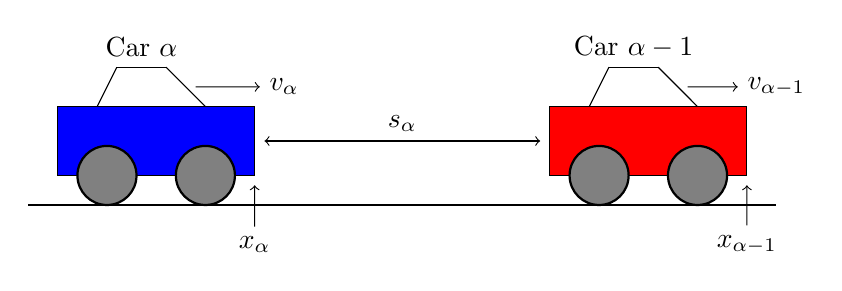
\begin{tikzpicture}[scale=1.25]
        \draw (-0.3,-0.3) -- (7.3,-0.3);
        \draw [fill = blue] (0,0) rectangle (2,0.7);
        \draw [fill=gray, thick] (0.5,0) circle [radius=0.3];
        \draw [fill=gray, thick] (1.5,0) circle [radius=0.3];
        \draw (1.5,0.7) -- (1.1,1.1);
        \draw (1.1,1.1) -- (0.6,1.1);
        \draw (0.6,1.1) -- (0.4,0.7);
        \node (car_a-1) at (0.85,1.3) {Car $\alpha$};
        \node (vel) at (2.3,0.9) {$v_{\alpha}$};
        \node (vel_start) at (1.3,0.9) {};
        \draw[->] (vel_start) -> (vel);
        \begin{scope}[shift={(5,0)}]
            \draw [fill = red] (0,0) rectangle (2,0.7);
            \draw [fill=gray, thick] (0.5,0) circle [radius=0.3];
            \draw [fill=gray, thick] (1.5,0) circle [radius=0.3];
            \draw (1.5,0.7) -- (1.1,1.1);
            \draw (1.1,1.1) -- (0.6,1.1);
            \draw (0.6,1.1) -- (0.4,0.7);
            \node (car_a-1) at (0.85,1.3) {Car $\alpha - 1$};
            \node (vel) at (2.3,0.9) {$v_{\alpha - 1}$};
            \node (vel_start) at (1.3,0.9) {};
            \draw[->] (vel_start) -> (vel);
          \end{scope}
        \node (x) at (2,0.35) {};
        \node (y) at (5,0.35) {};
        \node (x_pos) at (2,0) {};
        \node (x_sym) at (2,-0.7) {$x_{\alpha }$};
        \node (x_pos1) at (7,0) {};
        \node (x_sym1) at (7,-0.7) {$x_{\alpha - 1}$};
        \draw[<->] (x) -- node[above] {$s_{\alpha}$} (y);
        \draw[<-] (x_pos) -- (x_sym);
        \draw[<-] (x_pos1) -- (x_sym1);
        \end{tikzpicture} 
    \centering
    \caption{Defining index, position, velocity, and gap of a car.}
    \begin{itemize}
      \item $x_\alpha$, position of $\alpha$th car.
      \item $v_\alpha$, velocity of $\alpha$th car.
      \item $a_\alpha$, acceleration of $\alpha$th car.
      \item $s_\alpha$, gap of $\alpha$th car.
      \item Will denote the car $\alpha - 1$ by car $l$.
    \end{itemize}
\end{figure}  
\end{frame}

\begin{frame}
  \frametitle{Coupled Differential Equations}
  \begin{align*} 
    \odv{x_\alpha(t)}{t} &= v_\alpha (t), \\
    \odv{v_\alpha (t)}{t} &= a_{\rm mic} (s_\alpha, v_\alpha, v_l).
  \end{align*}
  Each car following model has a specific acceleration function: $a_{\rm mic} (s_\alpha, v_\alpha, v_l)$.
\end{frame}

\begin{frame}
  \frametitle{Full Velocity Difference Model}
  \begin{gather*}
      a_{\rm mic}(s_\alpha,v_\alpha,v_l) = \frac{v_{\rm opt} (s) - v_\alpha}{\tau} - \gamma \Delta v, \\
      v_{\rm opt} (s) = \max \left( 0, \min \left( v_0, \frac{s-s_0}{T} \right) \right).
  \end{gather*}
  \centerline{\rule{0.8\linewidth}{.2pt}}
  \begin{figure}[H]
    \begin{center}
      \begin{tabular}{c l c } 
      $v_0$ & desired speed  \\
      $s_0$ & minimum distance gap \\
      $T$ & time gap \\
      $\tau$ & speed adaptation time \\
      $\gamma$ & speed difference sensitivity \\
      \end{tabular}
      \end{center}
  \end{figure}
\end{frame}

\begin{frame}
  \frametitle{Optimal Velocity Function}
  \begin{figure}[H]
    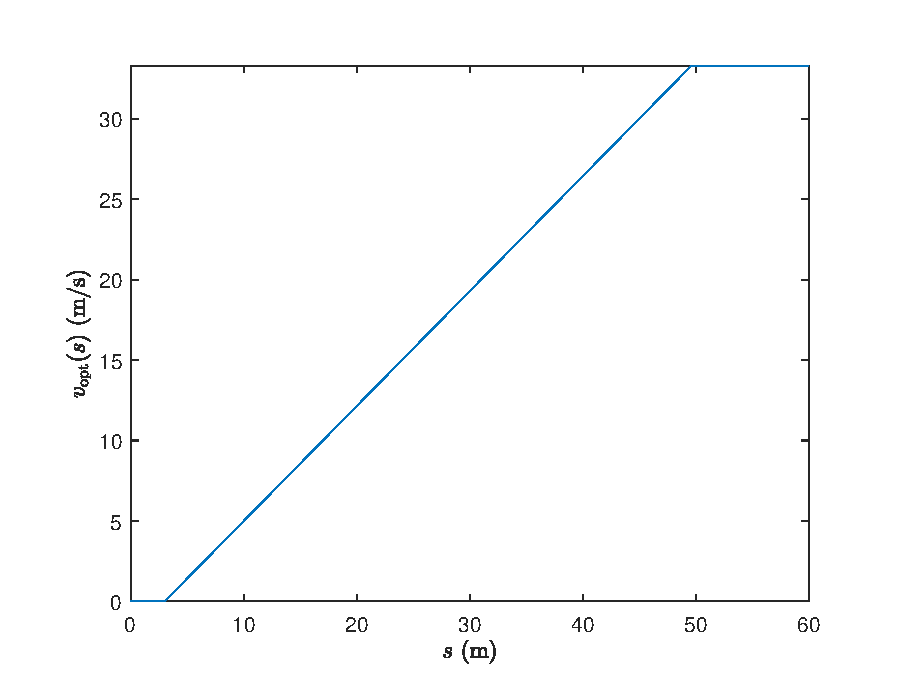
\includegraphics[width=9cm]{vopt_versus_s.eps}
    \centering
    \caption{Graph of the optimal velocity function over a range of gaps.}
\end{figure}
\end{frame}

\section{Implementation}
\begin{frame}
  \frametitle{Forwards Euler Method Scheme}
  During lane changes, the acceleration function is not continuous, so Euler's Method would be the most stable:
  \begin{align*}
    v_\alpha(t+\Delta t) &= v_\alpha(t) +a_{\rm mic}(s_\alpha(t), v_\alpha (t), v_l (t))\Delta t, \\
    x_\alpha(t + \Delta t) &= x_\alpha(t) + \frac{v_\alpha (t) + v_\alpha (t+\Delta t)}{2}\Delta t.
\end{align*}
\end{frame}

\begin{frame}
  \frametitle{Lane Changes}
  \begin{figure}[H]
    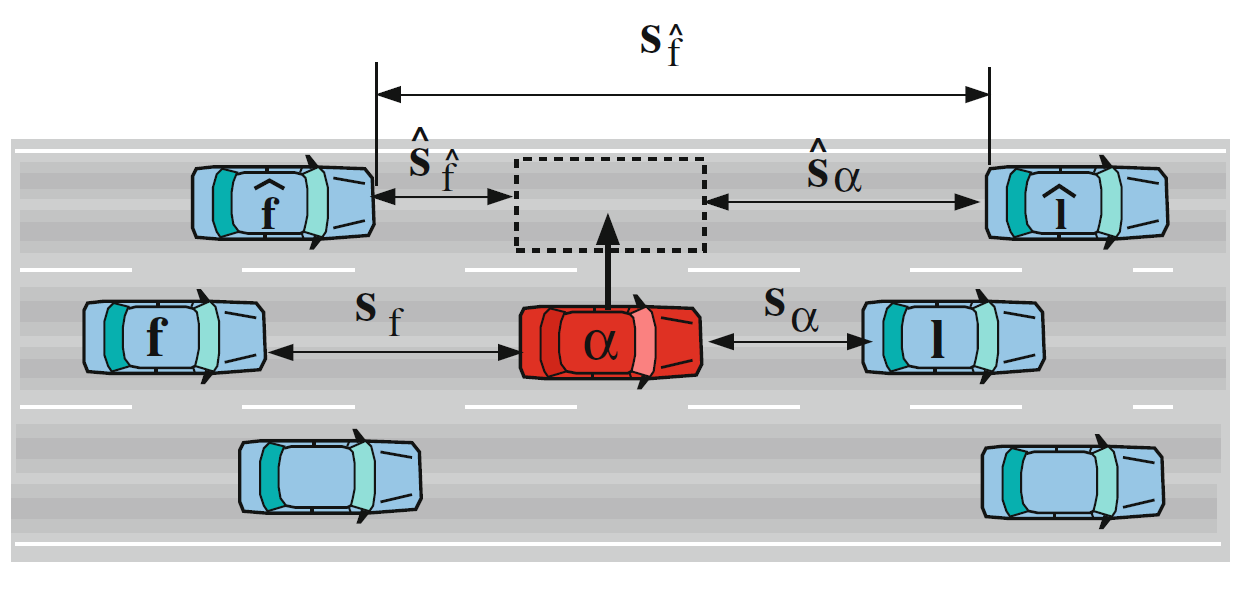
\includegraphics[width=8cm]{lane_change_diagram.PNG}
    \centering
    \caption{Multi-lane notation. From Treiber and Kesting \textit{Traffic Flow Dynamics}}
\end{figure}
  Define minimum $\hat s_{\hat f}$ and $\hat s_{\alpha}$ needed to change lanes: 
  \begin{align*}
    s_{\rm safe} (v_{\hat f}, v_{\alpha}) = v_{\rm opt}^{-1} \left[v_{\hat f} -\tau b_{\rm safe} + \tau \gamma (v_{\hat f} - v_{\alpha}) \right],\\
    s_{\rm adv} = s_{\alpha} + v_{\rm opt}^{-1} \left[\tau(\Delta a + a_{\rm bias} + \gamma(v_l - v_{\hat l}))\right].
  \end{align*}
\end{frame}

\begin{frame}
  \frametitle{Pseudocode for the FVDM}
  \begin{algorithm}
    \caption{Simplified algorithm for FDVM with lane changes}\label{alg:car-following-lane}
    \begin{algorithmic}
    \Require Initial state variables for each car at $t=0$. 
    \Require carArr, an array of cars.
    \For{$i = 1:$numsteps}{}
    \For{$j =$ length(carArr):$-1$:$1$}{}
      \State State variables of $j$th car $\gets$ Update $j$th car by a timestep.
      \State New lane of $j$th car $\gets$ carArr($j$).changeLane()
      \EndFor
      \State sort(carArr)
    \EndFor
    \end{algorithmic}
    \end{algorithm}
\end{frame}
\section{Examining Scenarios}

\subsection{Homogeneous Traffic}

\begin{frame}
  \frametitle{Homogeneous Traffic}
  \begin{figure}[H]
    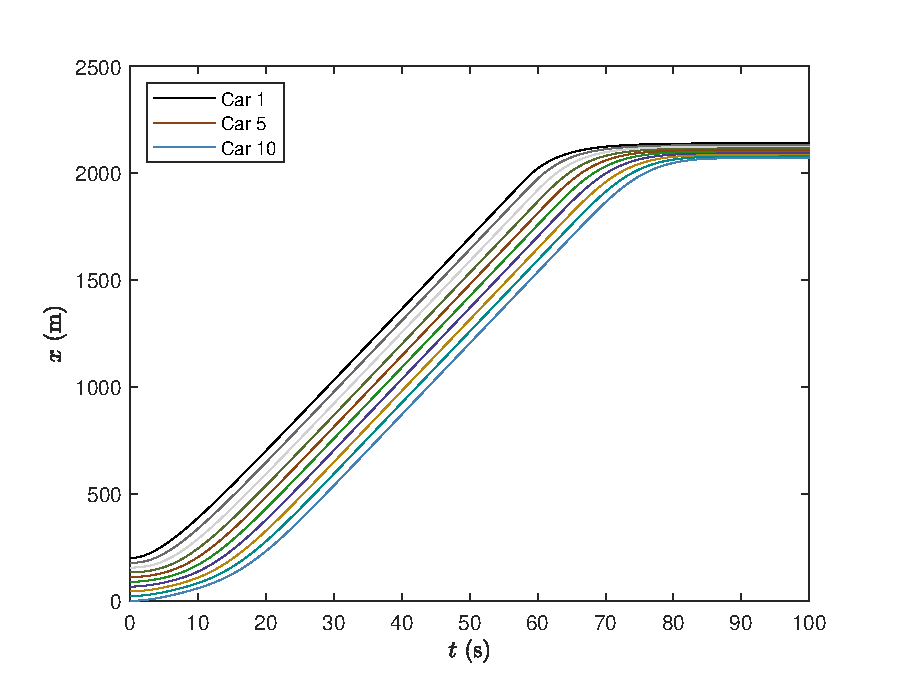
\includegraphics[width=8cm]{HomogeneousTraffic1.eps}
    \caption{Position versus time} 
\end{figure}
\end{frame}

\begin{frame}
  \frametitle{Homogeneous Traffic}
  \begin{figure}[H]
    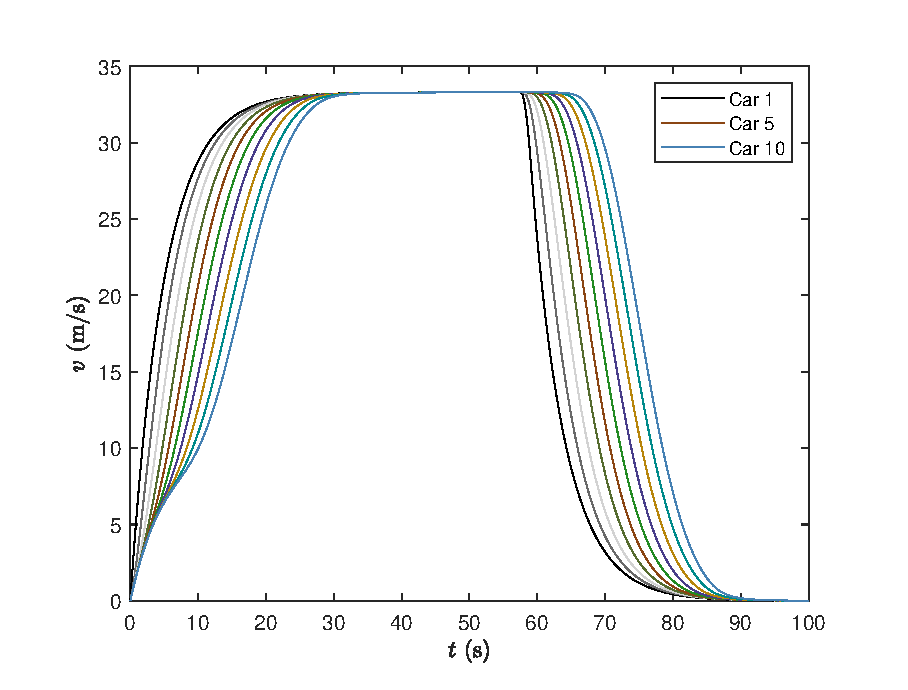
\includegraphics[width=8cm]{HomogeneousTraffic2.eps}
    \caption{Velocity versus time}
\end{figure}
\end{frame}

\begin{frame}
  \frametitle{Homogeneous Traffic}
  \begin{figure}[H]
    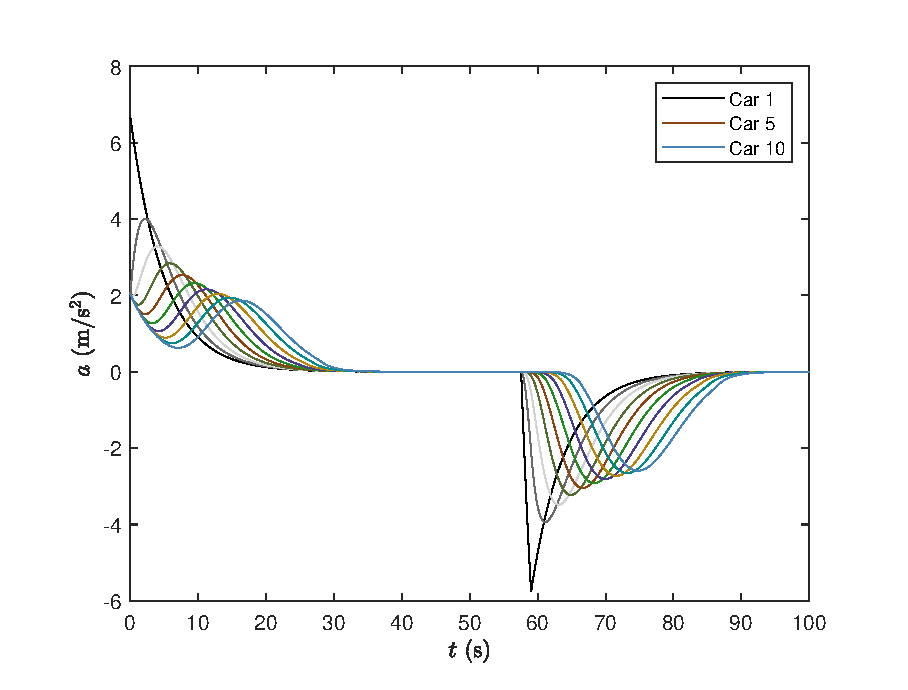
\includegraphics[width=8cm]{HomogeneousTraffic3.eps}
    \caption{Acceleration versus time}
\end{figure}
\end{frame}

\begin{frame}
  \frametitle{Homogeneous Traffic}
  \begin{figure}[H]
    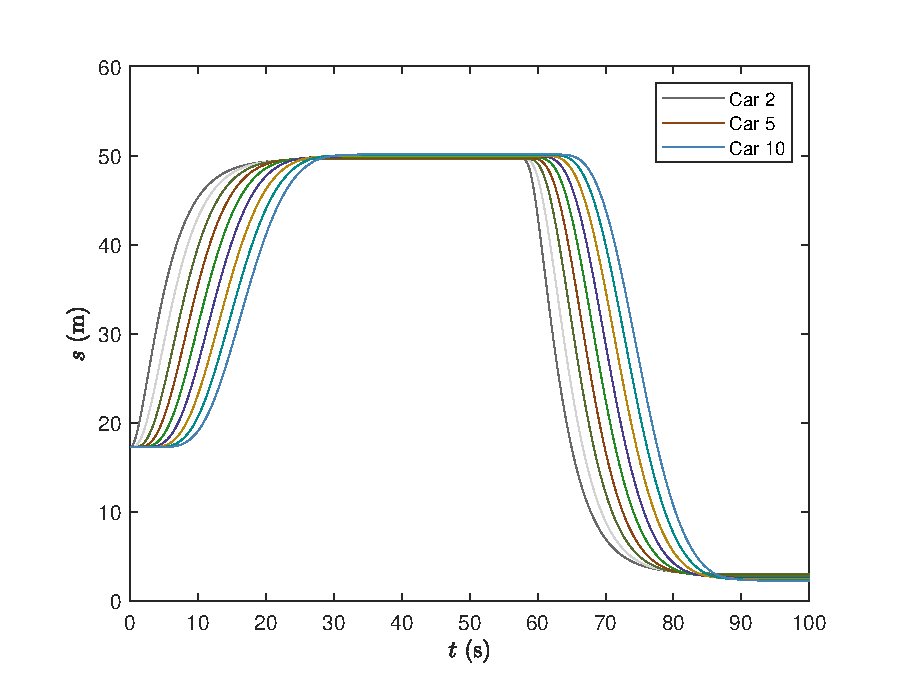
\includegraphics[width=8cm]{HomogeneousTraffic4.eps}
    \caption{Gap versus time}
\end{figure}
\end{frame}

\subsection{Obstacle}

\begin{frame}
  \frametitle{Obstacle}
  \begin{figure}[H]
    \includegraphics[width=8cm]{BottleNeck1.eps}
    \caption{Position versus time} 
\end{figure}
\end{frame}

\begin{frame}
  \frametitle{Obstacle}
  \begin{figure}[H]
    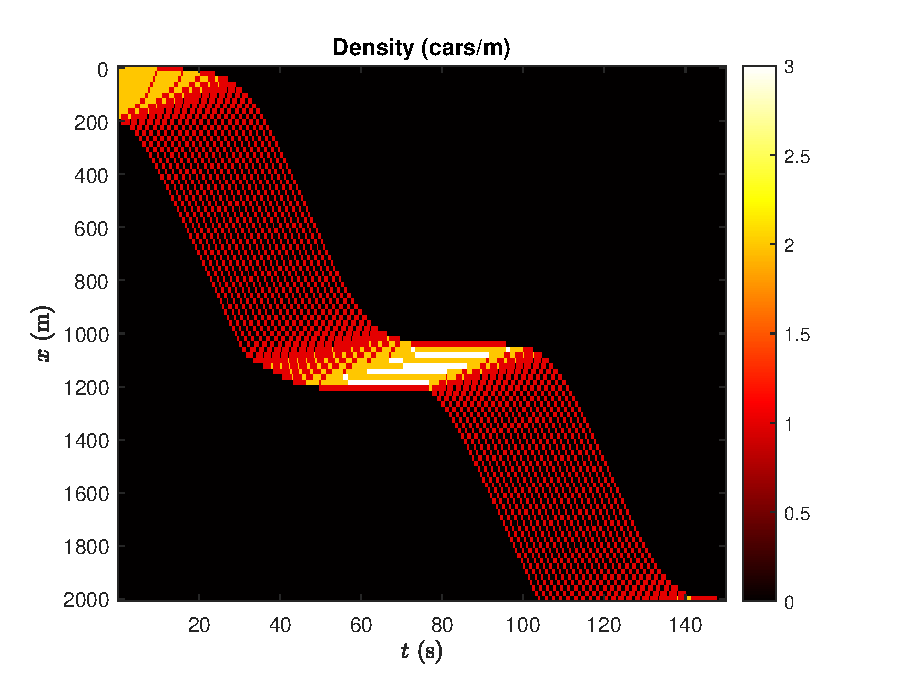
\includegraphics[width=5.5cm]{BottleNeck5.eps}
    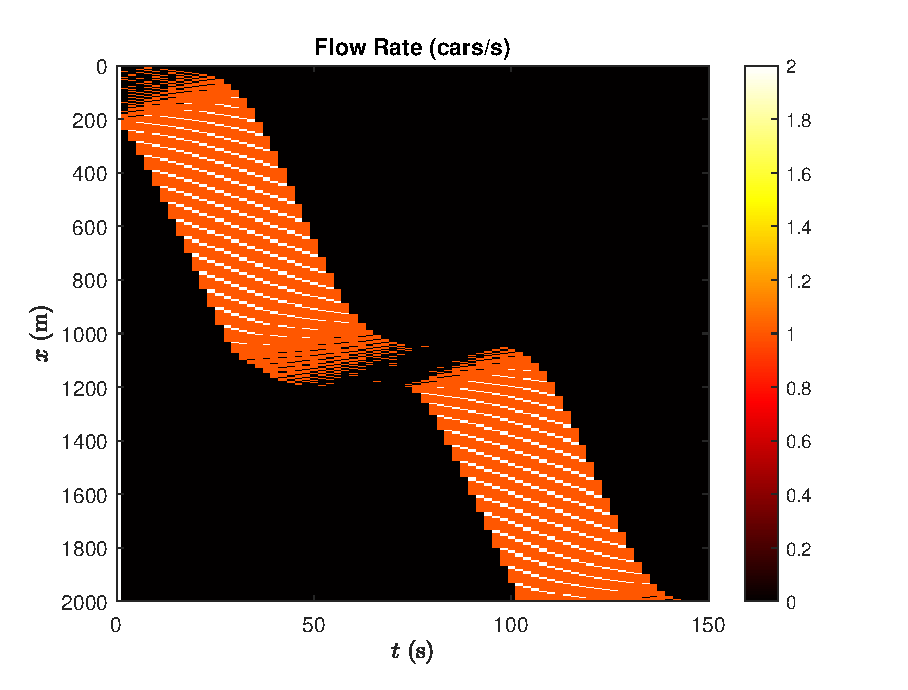
\includegraphics[width=5.5cm]{BottleNeck6.eps}
    \caption{Left to right: density vs time and distance; flow rate vs time and distance}
\end{figure}
\end{frame}

\begin{frame}
  \frametitle{Obstacle}
  \begin{figure}[H]
    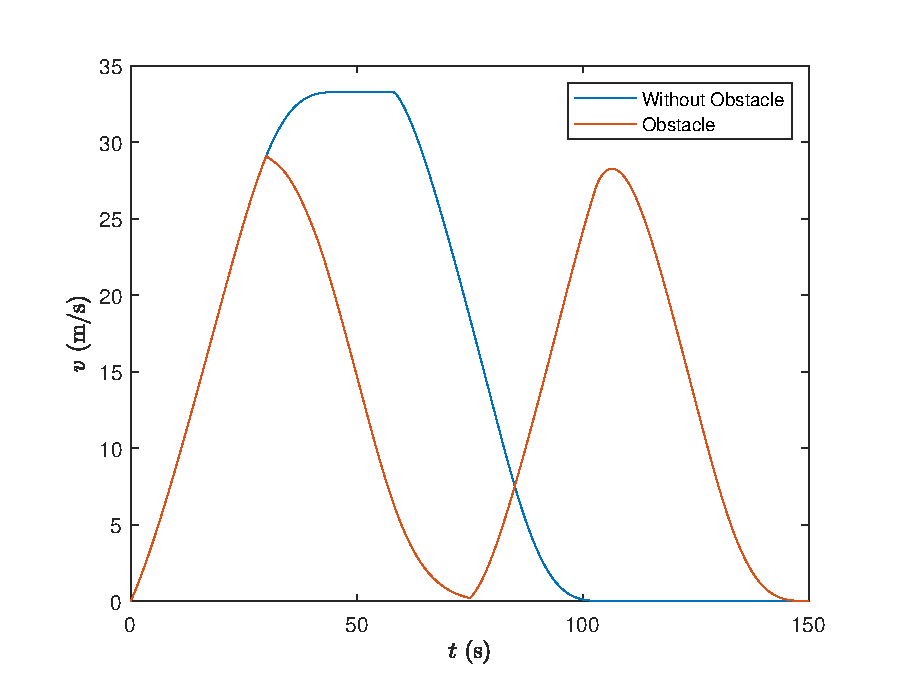
\includegraphics[width=8cm]{BottleNeck7.eps}
    \caption{Mean velocity of traffic with and without an obstacle.}
  \end{figure}
\end{frame}


\subsection{Multi-lane Bottleneck}

\begin{frame}
  \frametitle{Multi-lane Bottleneck}
  \begin{figure}[H]
    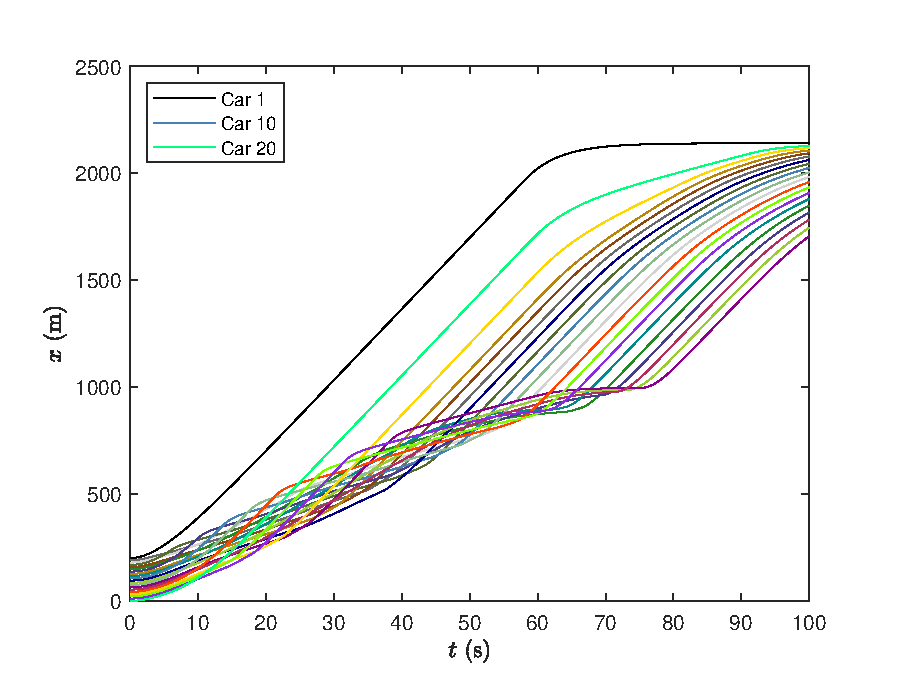
\includegraphics[width=8cm]{mlbn_x.eps}
\end{figure}
\end{frame}

\begin{frame}
  \frametitle{Multi-lane Bottleneck}
  \begin{figure}[H]
    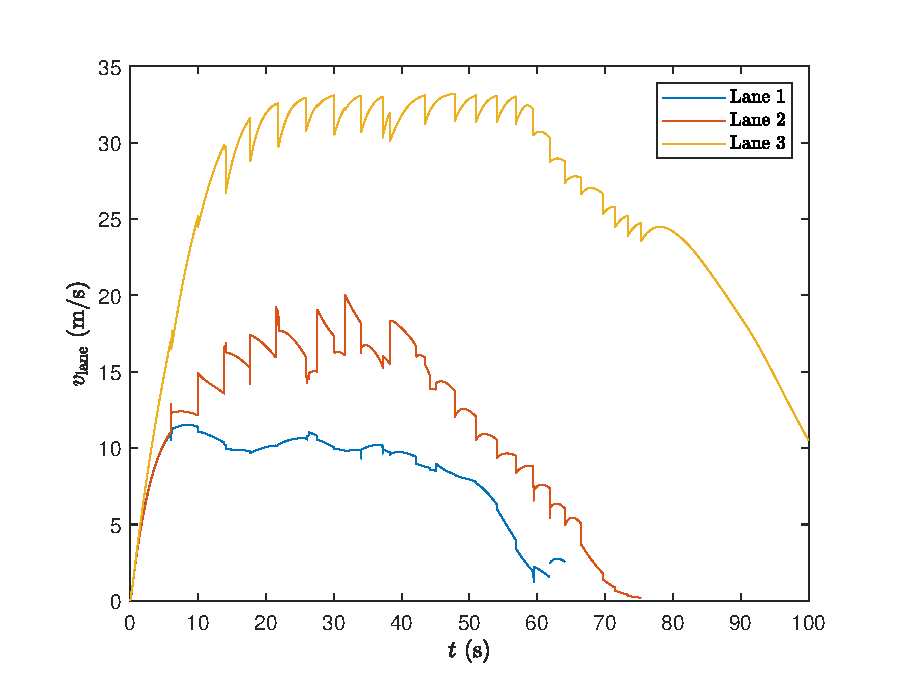
\includegraphics[width=5.5cm]{mlbn_laneSpeed.eps}
    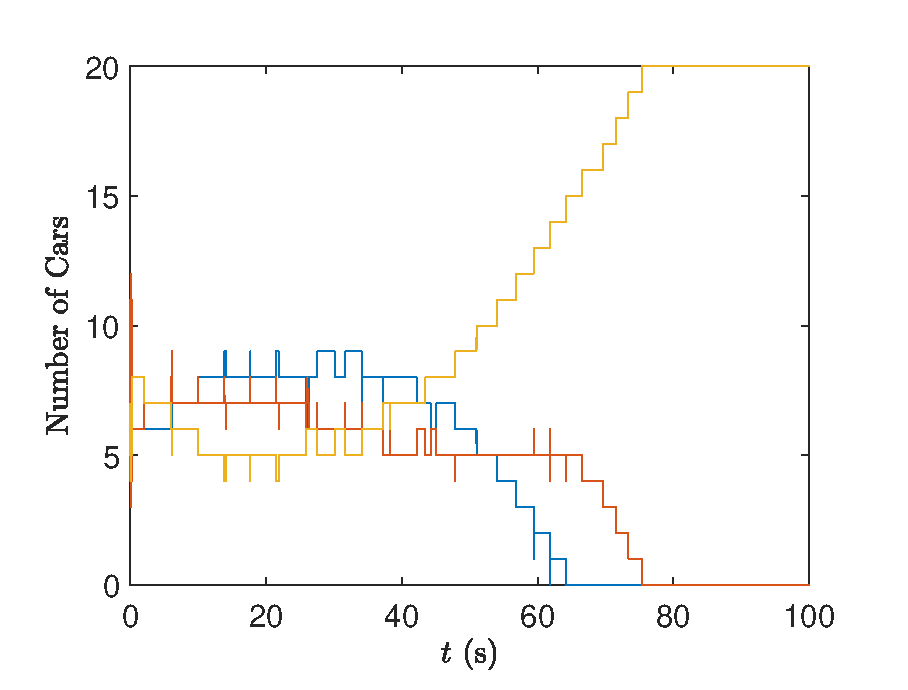
\includegraphics[width=5.5cm]{mlbn_lanecars.eps}
    \caption{Left to right: Mean velocity in each lane vs time; number of cars in each lane vs time}
\end{figure}
\end{frame}

\begin{frame}
  \frametitle{Multi-lane Bottleneck}
  \begin{figure}[H]
    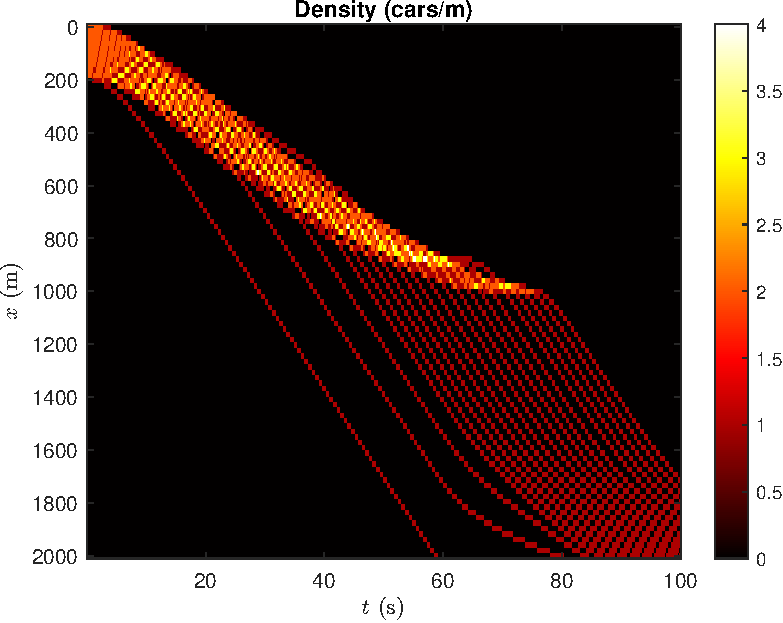
\includegraphics[width=5.5cm]{mlbn_density.pdf}
    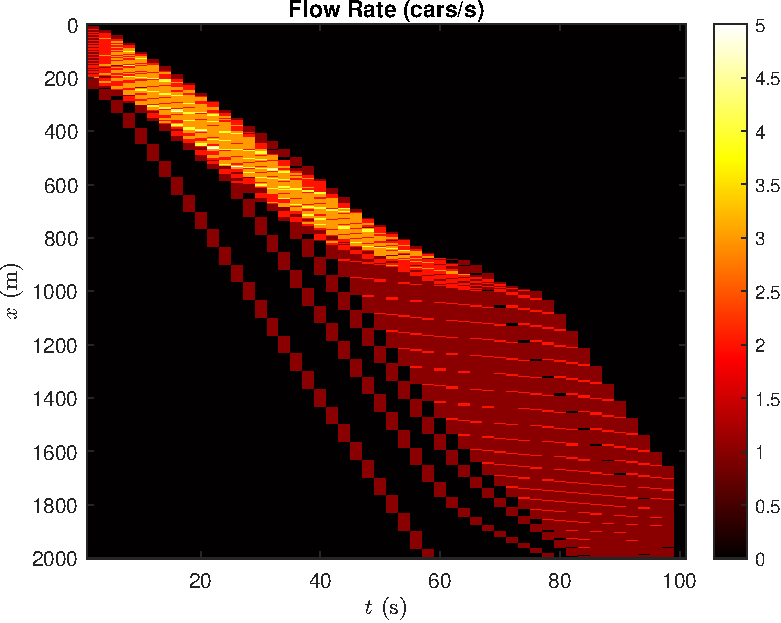
\includegraphics[width=5.5cm]{mlbn_flow.pdf}
    \caption{Left to right: density vs time and distance; flow rate vs time and distance}
\end{figure}
\end{frame}


\section{Conclusion}
\begin{frame}
  \frametitle{Conclusion}
  \begin{itemize}
    \item The FVDM with lane changes can model traffic flow and lets us examine how it can be interrupted by obstacles and bottlenecks. 

    \item Pitfalls in the model include unrealistic accelerations and erratic lane changes.
    
    \item Future work could model priority lanes and roundabouts
  \end{itemize}
\end{frame}
\end{document}